\documentclass[10pt, journal, a4paper]{IEEEtran} 

\usepackage[utf8]{inputenc}
\usepackage[T1]{fontenc}
\usepackage{amsmath, amssymb, amsfonts}
\usepackage{graphicx}
\usepackage{booktabs}
\usepackage{tabularx}
\usepackage{multirow}
\usepackage{hyperref}
\usepackage{float}
\usepackage{geometry}
% �� 引入 strip 宏包来支持双栏中的通栏大表格
\usepackage{cuted} 

% 根据要求设置边距：左、上 2.5 cm，右、下 2 cm [cite: 10]
\geometry{
    a4paper,
    top=2.5cm,
    left=2.5cm,
    right=2.0cm,
    bottom=2.0cm
}

\usepackage[style=ieee, backend=biber]{biblatex}
\addbibresource{references.bib}
\renewcommand*{\bibfont}{\footnotesize}

\title{\LARGE \bf Safety Performance Evaluation of Reinforcement Learning with Transformer Policies in Autonomous Driving}

\author{Jun Xuan Ng}

\begin{document}

\begin{strip}
\small
\begin{tabularx}{\textwidth}{|p{4.5cm}|X|}
\hline
\textbf{Article Info} & \textbf{ABSTRACT} (10 PT) \\ \hline
\vspace{0.5mm}
\textbf{\textit{Article history:}} \newline
Received Month dd, yyyy \newline
Revised Month dd, yyyy \newline
Accepted Month dd, yyyy & 
\multirow{2}{*}{\parbox{\linewidth}{%
\vspace{1.5mm}
% !TeX root = ../main.tex

\begin{abstract}
This paper systematically evaluates the performance of the ViT model algorithm based on SAC at unsignalized intersections in the CARLA simulator. Although reinforcement learning has shown potential in autonomous driving tasks, the performance of ViT at unsignalized intersections remains unclear. This study concludes by finding that the ViT model still has significant room for improvement at unsignalized intersections, and adjusting hyperparameters can significantly improve the control strategy. This research provides valuable experience for the performance of Transformer-based models at unsignalized intersections and lays the foundation for future vision-based autonomous driving models.
\end{abstract}

\begin{IEEEkeywords}
Autonomous Driving, Deep Reinforcement Learning, Transformer, Safety Performance, Systematic Literature Review
\end{IEEEkeywords}
\vspace{2mm}
}} \\ 
\cline{1-1} 
\vspace{0.5mm}
\textbf{\textit{Keywords:}} \newline
Autonomous driving, \newline
Deep reinforcement learning, \newline
Vision Transformer, \newline
Soft Actor-Critic, \newline
Unsignalized intersections, \newline
Traffic safety & \\ \hline

\multicolumn{2}{|p{16.5cm}|}{%
\vspace{0.5mm}
\centering \scriptsize \textit{This is an open access article under the CC BY-SA license.}
\vspace{0.5mm}} \\ \hline
\textbf{Corresponding Author:} & Jun Xuan Ng, \textit{School of Computing, Multimedia University, Email: your.email@example.com} \\ \hline
\end{tabularx}
\vspace{5mm}
\end{strip}

% !TeX root = ../main.tex

\section{introduction}
    \subsection{background of the Study}
    Since OpenAI released its ChatGPT chatbot model in 2022 \cite{noauthor_introducing_2022}, there has been growing recognition of the potential of AI and increasing attention to AI-related fields. Currently, the success of AI is largely attributed to Google's Transformer model released in 2017: the attention mechanism is key \cite{vaswani_attention_2023}. While the performance of the Transformer is undeniable, it is a data-intensive model. Compared to simpler models (such as convolutional neural networks (CNNs)), the Transformer requires significantly more data to outperform CNNs. Reinforcement learning effectively addresses the problem of data scarcity. It allows the model to interact with its environment, generating more data and thus compensating for the lack of sufficient data.

    In intelligent vehicle engineering, the technical approach of combining self-attention mechanisms with deep reinforcement learning (DRL) has shown strong application potential in multiple fields.

    \cite{huang_research_2025} has demonstrated that self-attention mechanisms can efficiently process inputs from multiple sensors with different perspectives. This allows autonomous driving systems to have a broader field of view to handle highly complex scenes. Meanwhile, rule-based algorithms often exhibit significant vulnerability when encountering complex dynamic spaces. To overcome this limitation, the highly nonlinear "Next Best View Problem" was perfectly solved through the Actor-Critic deep reinforcement learning mechanism and model autonomous exploration, achieving high-precision 3D point cloud environment digital mapping \cite{menglong_yang_automatic_2019}.

    Although previous studies have demonstrated the "powerful spatial modeling capability of self-attention mechanisms in continuous pixel parsing" \cite{huang_research_2025} and the "excellent performance of deep reinforcement learning agents in chassis physical trajectory exploration" \cite{menglong_yang_automatic_2019}, the exploration of how to perfectly decouple and integrate spatiotemporal Vision Transformer (ViT) with maximum entropy continuous control reinforcement learning (SAC) at unsignalized intersections remains very limited in the academic community.

    To completely fill this critical academic gap, this study makes a theoretical contribution to the field of autonomous driving, enriches the literature on using attention mechanisms for robot decision-making, and proves that reinforcement learning can effectively train Transformer models, thereby overcoming the problem of data scarcity.

    \subsection{Objective of Research}
    \begin{enumerate}
        \item To develop a ViT model as the core model for this research. 
        \item To combine the soft Actor-Critic (SAC) algorithm with the ViT architecture to construct a deep reinforcement learning decision framework. 
        \item To evaluate the performance and feasibility of ViT-SAC in unsignalized intersection using metrics such as success rate and collision rate.
    \end{enumerate}

    \subsection{Research Question}
    \begin{enumerate}
        \item In a simulation environment, to what extent can the Soft Actor-Critic (SAC) algorithm alleviate the data requirements of the Transformer model through autonomous exploration and experience replay?
        \item In CARLA, how does integrating a ViT-based policy network affect the convergence speed and stability of the reinforcement learning process?
        \item How do the success rate and collision rate perform when using SAC to handle multi-agent interactions at unsignalized intersections?
    \end{enumerate}

% !TeX root = ../main.tex

\section{Literature Review}
    In 2024, \cite{elallid_improving_2024} proposed an autonomous driving framework combining ViT and SAC. Their ViT-SAC model was trained using 13,542 human expert demonstration data samples for imitation learning. The framework was evaluated in the CARLA simulator under different traffic densities (up to 210 vehicles) at roundabouts and right-turn intersections. The results showed a 100\% success rate with no collisions at roundabouts; at peak density at right-turn intersections, their success rate reached 96\%, significantly outperforming standard SAC, PPO, and DQN baselines.

    \subsection{ViT}
    \cite{dosovitskiy_image_2021} demonstrated that the Vision Transformer (ViT) achieved excellent results in computer vision tasks. Compared to Convolutional Neural Networks (CNNs), ViT's advantage lies in its global perspective. CNNs are like a blind person using a magnifying glass to see an image; shallow networks can only see local pixels, and multiple layers must be stacked to see the whole picture. However, ViT's self-attention mechanism allows it to establish connections between all pixels in the entire image from the first layer. The downside is that ViT is a data-hungry model, requiring more data to outperform CNNs.

    \subsection{SAC}
    Soft Actor-Critic (SAC) was proposed in \cite{haarnoja_soft_2018}. It is an offline deep reinforcement learning algorithm based on maximum entropy reinforcement learning and the stochastic Actor-Critic algorithm. It is suitable for tasks requiring a continuous action space. SAC uses one Actor network and two Q-function networks, which can also be considered as critics. The output of the Actor network is the parameters (mean and standard deviation) of the action probability distribution. In short, the two critics evaluate the Actor's behavior. The critic learns from the actor's actions and feedback from the environment.

    \subsection{Performance Comparison}
    \begin{table}[htbp]
    \centering
    \caption{Comparative Performance Analysis of Unsignalized Intersection}
    \label{tab:comparative_performance}
    \begin{tabularx}{\linewidth}{lXlll}
    \toprule
    \textbf{Ref.} & \textbf{Input Type} & \textbf{Algorithm} & \textbf{Collision Rate} & \textbf{Success Rate}\\
    \midrule
    \cite{r_zhao_autonomous_2025} & Position and speed for surrounding vehicle and Return-to-cost & PPO & $64\%$ & $-$ \\
    \addlinespace
    \cite{doroudian_balancing_2024} & Position and speed for surrounding vehicle & PPO & $2\%$ & $98\%$ \\
    \addlinespace
    \cite{zhao_constraint-guided_2024} & Position and speed for surrounding vehicle & PPO/TD3 & $64.26\% / 66.73\%$ & $-$ \\
    \addlinespace
    \cite{x_zhang_integrating_2025} & Front-view Images & SAC & $25.7\%$ & $67.3\%$ \\
    \addlinespace
    \cite{liu_mtd-gpt_2023} & Position and speed for surrounding vehicle & PPO & $-$ & $94\%$ \\
    \addlinespace
    \cite{kargar_vision_2022} & Bird Eye’s View (BEV) & DQN & $5\%$ & $-$ \\
    \addlinespace
    \cite{elallid_improving_2024} & Front-view Images & SAC & $0\%$ & $100\%$ \\
    \bottomrule
    \end{tabularx}
    \end{table}

    \ref{tab:comparative_performance} shows existing literature and research results. The experimental scenarios in these studies are all unsignaled traffic intersections, similar to this study. The collision rate and success rate metrics are summarized here.

    \ref{tab:comparative_performance} shows that most studies use low-dimensional data as input, such as the position and speed information of other vehicles. However, this study uses high-dimensional front view images as input. This is more challenging than tasks using low-dimensional data as input. \cite{elallid_improving_2024} and \cite{kargar_vision_2022} have similar data input types to this study. \cite{elallid_improving_2024} is also the main reference paper for this study.

    This study will use front view images as input, similar to \cite{elallid_improving_2024}. Although \cite{kargar_vision_2022} also uses visual data as input, it uses a bird's-eye view. Compared to a bird's-eye view, a front view image is more practically applicable.
    
\newpage
% % !TeX root = ../main.tex

\section{Methodology}
    \subsection{Observation Space}
    This study will use three cameras as input because intersection scenes require a wider field of view (FOV). 

    The target point is projected onto the vehicle's local coordinate system using a rotation matrix based on the current yaw angle:

    \begin{align*}
    lx &= dx \cdot \cos(-\psi) - dy \cdot \sin(-\psi) \\
    ly &= dx \cdot \sin(-\psi) - dy \cdot \cos(-\psi)
    \end{align*}

    \begin{table}[htbp]
    \centering
    \caption{Specification of Observation Components and Shapes.}
    \label{tab:observation_shapes}
    \begin{tabular}{lll}
    \toprule
    \textbf{Component} & \textbf{Shape} & \textbf{Range} \\
    \midrule
    Visual & $[4(\text{Frame}), \text{Height}, 3(n_{\text{camera}}) \times \text{Width}, 3(\text{RGB})]$ & $[0, 255]$ \\
    \addlinespace
    Goal   & $[2(\text{goal vector})]$ & $[-\infty, \infty]$ \\
    \bottomrule
    \end{tabular}
    \end{table}

    Here are some other parameters related to the camera:

    \begin{table}[htbp]
    \centering
    \caption{Camera Hyperparameters.}
    \label{tab:cam parameters}
    \begin{tabular}{ll}
    \toprule
    \textbf{Component} & \textbf{Value} \\
    \midrule
    Pixel & $[56\times56]$ \\
    \addlinespace
    FOV   & $60\degree$ \\
    \addlinespace
    Position & $[x=1.5,y=0,z=2]$ \\
    \bottomrule
    \end{tabular}
    \end{table}
    
    \subsection{Action Space}
    \cite{corrado_simulation-acquired_2022} pointed out that reinforcement learning requires a large number of interactions to converge in high-dimensional continuous control problems. By introducing a mapping mechanism to compress the high-dimensional action space into a low-dimensional latent action space, the data utilization efficiency and convergence speed of the agent can be directly improved. In this study, I simplified the three action spaces in \cite{elallid_improving_2024} into two action spaces: acceleration and steer.

    \begin{table}[htbp]
    \centering
    \caption{Specification of Action Components and Shapes.}
    \label{tab:action_shapes}
    \begin{tabular}{lll}
    \toprule
    \textbf{Component} & \textbf{Range} \\
    \midrule
    Steering & $[-1.0, 1.0]$ \\
    \addlinespace
    Acceleration/Brake  & $[-1.0, 1.0]$ \\    \bottomrule    
    \end{tabular}
    \end{table}

    \subsection{Reward feedback}
    The reward in this study is divided into three parts: 
    The global reward function $\mathcal{R}_{\text{total}}$ is structured hierarchically as formulated in Equation \ref{eq:total_reward}:
    \begin{equation}
        \mathcal{R}_{\text{total}} = \mathcal{R}_{\text{sparse}} + \mathcal{R}_{\text{shaping}} + \mathcal{R}_{\text{fine}}
        \label{eq:total_reward}
    \end{equation}
    \subsubsection{Sparse Reward}
    This reward is crucial to success or failure, directly determining the end of the round.

    When the agent safely reaches its destination, it receives a substantial termination sparse reward of $\mathcal{R}_{\text{success}} = +10.0$. Conversely, if the agent collides or leaves the road during the process, it will suffer a severe penalty of $\mathcal{R}_{\text{collision}} = \mathcal{R}_{\text{offroad}} = -10.0$.
    
    \subsubsection{Shaping Reward}
    To mitigate the typical vanishing policy gradient defect caused by purely sparse signals, the system introduces continuously shaping parameters to guide the model for efficient intersection crossing tracking.

    The distance reward $\mathcal{R}_d$ measures the decrease in physical Euclidean distance to the target between consecutive time steps $t-1$ and $t$. In the code execution of this study, this displacement value is first scaled down by a factor of 10 (multiplied by 0.1) to perform standard reward scaling, and then scaled up by a factor of 5 (multiplied by 5) to make the target more attractive to the agent, ultimately forming the form $\mathcal{R}_d = 0.5 \times (d_{t-1} - d_t)$. Meanwhile, the velocity reconstruction reward $\mathcal{R}_v$ undergoes bimodal optimization: to prevent the policy network from becoming overly conservative and stuck in place, any velocity below $0.5 \text{ m/s}$ triggers a dynamic penalty; for a compliant cruising speed profile, the policy is guided by a reward of $\min(v_t, 10.0) / 33.0$, capped at 10 m/s. This boundary setting is based on the evaluation results of \cite{elallid_improving_2024} on a right-turn baseline (this paper validates that the average tactical speed does not exceed $5 \text{ m/s}$ in complex intersection right-turn scenarios).
    
    \subsubsection{Fine Tune Reward}
    To prevent aberrant agent behavior such as sudden lane changes or illegal shortcuts, this study explicitly introduces micro-adjustment penalties as defined in the formula \ref{eq:total_reward}. Driving on or crossing a dashed line triggers a slight penalty of $\mathcal{R}_{\text{marking}} = -0.025$. Intruding into or driving in the oncoming lane represents a high risk and therefore triggers a severe risk-avoidance penalty of $\mathcal{R}_{\text{oncoming}} = -0.200$. This specific mathematical asymmetry (meaning the penalty for driving on the wrong side of the road is much greater than the penalty for crossing a dashed line) forces the policy gradient to strictly prioritize lane centering and adherence to standard traffic regulations, thereby ensuring vehicles navigate unsignaled intersections with elegant dynamic trajectories and compliant legal behavior.

    \subsection{Condition}
    The following are the triggering conditions for this study:

    \textbf{1) Collision Telemetry:} The collision signal is emitted by the collision sensor integrated in CARLA.

    \textbf{2) Oncoming Lane Invasion (Otherlane flag):} This study constructs a two-dimensional vector orientation alignment mechanism as shown in the formula \ref{eq:dot_product}. The simulation environment extracts the horizontal forward orientation vector $\mathbf{v}_{\text{ego}}$ of the main vehicle in real time and performs an algebraic dot product calculation with the legal driving direction vector $\mathbf{v}_{\text{lane}}$ mapped to the local lane heading point. When the scalar is positive (dot product > 0), it means the vehicle's direction is within the compliant envelope of $\pm 90^{\circ}$. Conversely, when the scalar is negative (dot product < 0), it indicates that the angle between the two vectors exceeds $90^{\circ}$, and the system will immediately trigger `otherlane flag` and activate the wrong-way penalty $\mathcal{R}_{\text{oncoming}}$.

    \textbf{3) Lane Marking Straddling (On marking flag):} When the spatial deviation between the vehicle's center coordinates and the lane centerline exceeds a critical threshold of approximately $1.40 \text{m}$, `on marking flag` will be triggered, identifying that the wheels have either touched or crossed the dashed line.

    \textbf{4) Roadway Departure (Off road flag):} When the sustained lateral deviation further increases to $\vert \Delta y \vert \ge 2.25 \text{ m}$, the system will determine that the vehicle has catastrophically left the road. Given that the physical width of the main body is approximately $2.0 \text{ m}$, a lateral offset of $2.25 \text{ m}$ mathematically means that more than $50\%$ of the vehicle's volume has crossed the solid road boundary, causing the vehicle to enter non-drivable areas such as grass, shoulders, or sidewalks.

    The directional alignment for oncoming lane invasion is mathematically formalized via the dot product of the vehicle's directional vectors:
    \begin{equation}
        \text{Invasion Trigger} = 
        \begin{cases} 
          \text{True (Otherlane\_flag)}, & \text{if } \mathbf{v}_{\text{ego}} \cdot \mathbf{v}_{\text{lane}} < 0 \\
          \text{False}, & \text{if } \mathbf{v}_{\text{ego}} \cdot \mathbf{v}_{\text{lane}} \ge 0
       \end{cases}
       \label{eq:dot_product}
    \end{equation}
    where $\mathbf{v}_{\text{ego}} = [x_{\text{ego}}, y_{\text{ego}}]^T$ and $\mathbf{v}_{\text{lane}} = [x_{\text{lane}}, y_{\text{lane}}]^T$ represent the localized 2D horizontal components of the ego vehicle's forward heading vector and the regulatory lane waypoint direction vector, respectively.
    
    Concurrently, the tracking boundary deviations $\Delta y$ from the idealized lane centerline dictate the micro-behavioral and structural failure states:
    \begin{equation}
        \text{State Status} = 
        \begin{cases} 
          \text{On\_marking\_flag}, & \text{if } 1.40 \text{ m} \le \vert \Delta y \vert < 2.25 \text{ m} \\
          \text{Off\_road\_flag}, & \text{if } \vert \Delta y \vert \ge 2.25 \text{ m}
       \end{cases}
    \end{equation}
    
    \subsection{Model Architecture}
    \subsubsection{Vision Transformer}
    \begin{figure}[t]
        \centering
        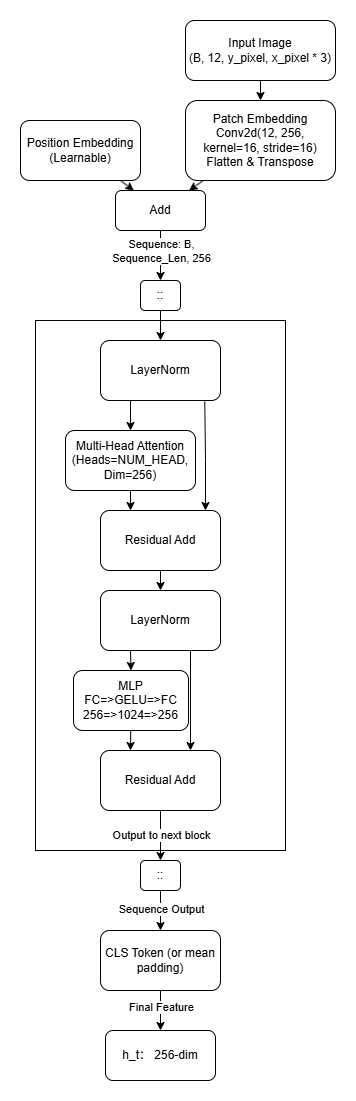
\includegraphics[width=0.3\textwidth]{figures/vit.png}
        \caption{The architectural visualization of Vision Transformer.}
        \label{fig:Vision Transformer Model}
    \end{figure}
    
    \ref{fig:Vision Transformer Model} show the architecture of the Vision Transformer network. The input shape of the ViT model in this study is $(B, 12, y_{pixels}, x_{pixels}\times3)$. $B$ is the batch size, and $12$ represents $3$ (RGB) × $4$ (frames). On the left is a learnable position embedding that adds positional information to each image patch. This helps the model identify the top-left and bottom-right image patches \cite{elallid_improving_2024}. The internal structure of the Transformer consists of 2 blocks and 8 heads. Finally, the output of ViT is a vector representing the "semantics of the entire image". This study uses the first label as the output. The final output is a 256-dimensional embedding feature vector. This vector will be used as state input for SAC (Soft Actor-Critic) algorithm to determine whether to "accelerate" or "brake".
    
    \subsubsection{Actor}
    \begin{figure}[t]
        \centering
        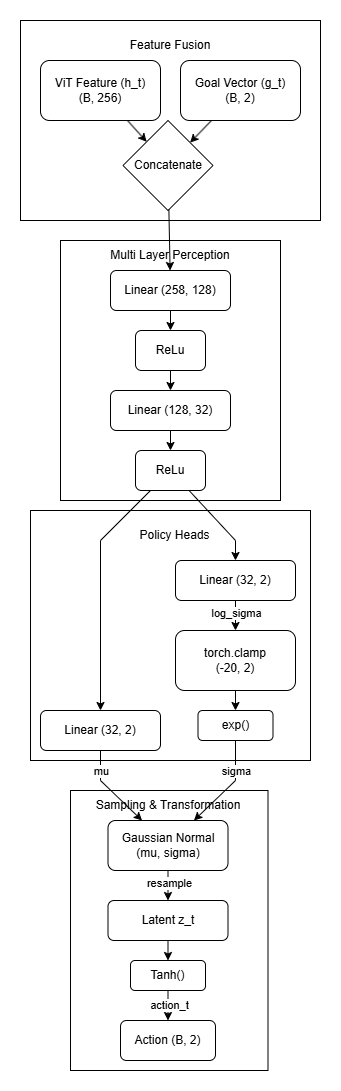
\includegraphics[width=0.3\textwidth]{figures/actor.png}
        \caption{The architectural visualization of Actor.}
        \label{fig:Actor architecture}
    \end{figure}
    \ref{fig:Actor architecture} show the architecture of the Actor. It combines the vector features output by ViT with the target vector and compresses it from 258 dimensions to 128 dimensions, and then further to 32 dimensions. The goal of this stage is to extract core signals from the fused features sufficient to determine driving behavior. Next comes probabilistic distribution modeling (policy head). The network branches here, outputting two parameters of a Gaussian distribution: mean ($\mu$): representing the ideal action center perceived by the model; standard deviation ($\sigma$): representing uncertainty or exploratory tendency in decision-making.
    
    \subsubsection{Double Critic}
    \begin{figure}[t]
        \centering
        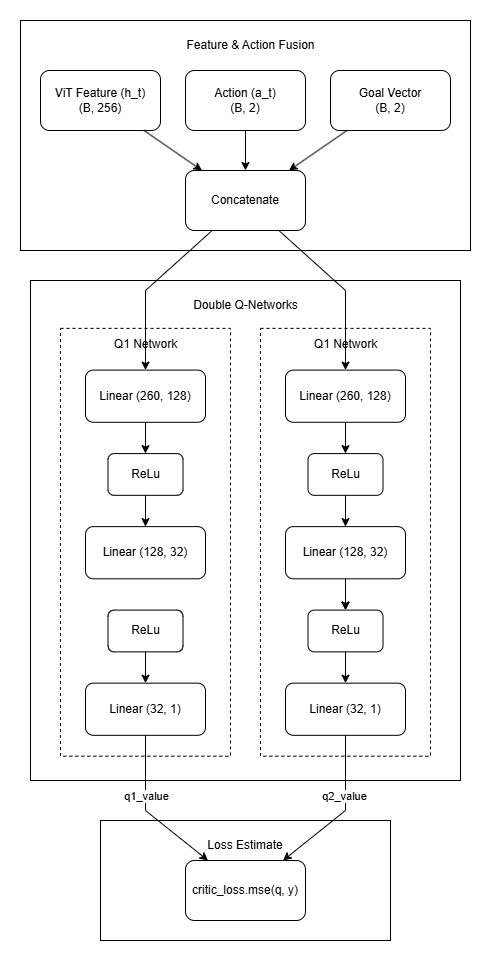
\includegraphics[width=0.3\textwidth]{figures/double critic.png}
        \caption{The architectural visualization of Critic.}
        \label{fig:Double Critic}
    \end{figure}
    \ref{fig:Double Critic} is a structure consisting of two evaluation networks. The first step is to concatenate the feature vector from the ViT output, target vector, and action, and then input the concatenated result into the two evaluation networks. Each channel in the evaluation network contains two fully connected layers (linear 260 $\pm$ 128 $\pm$ 32) with ReLU nonlinear activation. Finally, the error between the two evaluator outputs is calculated as a mean squared error (MSE) function, the results are summed, and then the network is updated.
    
    \subsubsection{Overview}
    \begin{figure}[t]
        \centering
        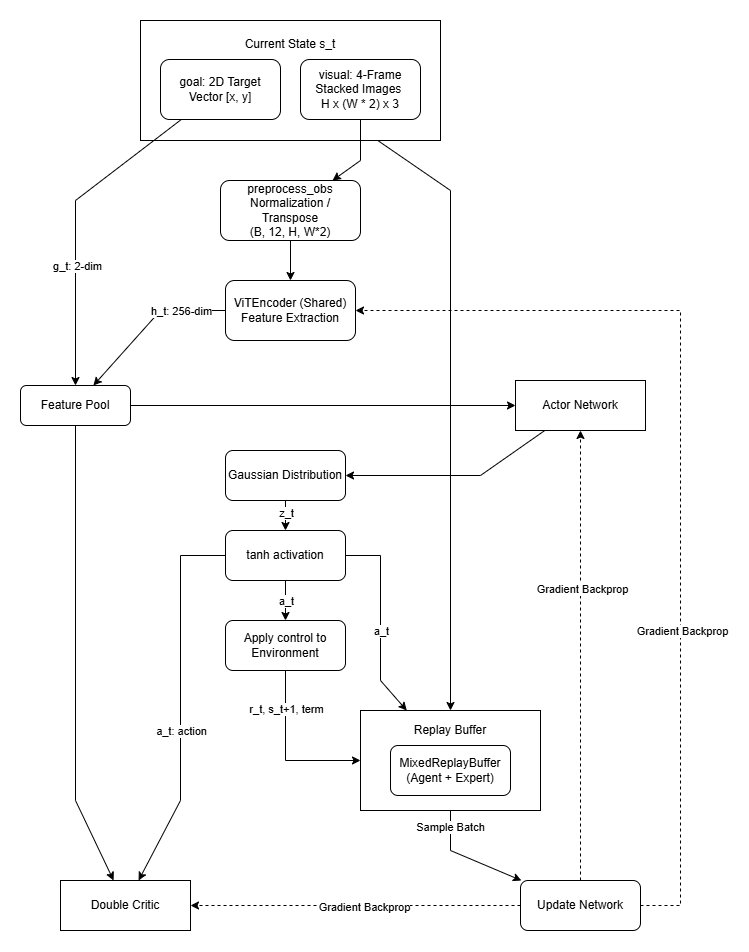
\includegraphics[width=0.3\textwidth]{figures/overview.png}
        \caption{Overview of the Model}
        \label{fig:Overview}
    \end{figure}
    \ref{fig:Overview} is the training workflow of the proposed ViT-SAC framework in this study.

    Perceptual Instantiation and Latent Space Encoding: Initially, the CARLA simulation environment instantiates the original state-space observation vector $\mathcal{S}_t$, which encapsulates the target vector and the original multi-camera, multi-frame visual pixel stream. The visual tensor undergoes normalization and resizing before being injected into the Vision Transformer (ViT) spatial encoder. ViT maps the high-dimensional visual input to a $256$-dimensional latent visual feature vector, which is temporarily archived in the structured feature library of the policy network.

    Random Action Generation and Boundary Constraints: Given that traffic light-free intersection navigation represents a highly complex task, the random actor network does not directly generate actions (steer and acceleration). Instead, the output of the policy head is a mean vector $\mu_t$ and a log-standard deviation vector $\log\sigma_t$ that can represent a Gaussian probability distribution. The system samples a potential action vector $z_t \sim \mathcal{N}(\mu_t, \sigma_t^2)$ based on a Gaussian probability distribution. The action vector is: $a_t = \tanh(z_t) \in [-1.0, 1.0]^2$. The two-dimensional output here represents the lateral steering torque and the longitudinal acceleration/braking command.

    Environmental Interaction: By executing $a_t$, the autonomous vehicle will interact with the CARLA environmental intersection and receive corresponding feedback (rewards or penalties). For example, a severe termination safety penalty of $-10.0$ is backpropagated when an adversarial collision telemetry signal is triggered.

    Asynchronous Experience Archive: The collected individual transition tuples—including the historical state $\mathcal{S}_t$, action $a_t$, environmental feedback (reward and penalty) $\mathcal{R}_{\text{total}}$, next state $\mathcal{S}_{t+1}$, and episode termination flag—are appended to \texttt{MixedReplayBuffer}. During concurrent training, the system samples mini-batch samples from this buffer to train and update the dual Critic network and Actor policy network. This single-step interaction pipeline is repeated over millions of temporal environmental steps.
    
    \subsubsection{Hyperparameter}
    \begin{table}[htbp]
    \centering
    \caption{The hyperparameters of this study}
    \label{tab:hyperparameter}
    \begin{tabular}{llc}
    \toprule
    \textbf{Notation} & \textbf{Meaning} & \textbf{Value} \\ \midrule
    $v_{max}$ & Velocity upper limit & 10 \\
    $v_{min}$ & Velocity lower limit & 0.5 \\
    $\gamma$ & Discount rate & 0.99 \\
    $N_{buffer}$ & Agent buffer capacity & 200000 \\
    $N_{A}$ & Agent buffer mini-batch size & 32 \\ 
    $N_{E}$ & Expert buffer mini-batch size & 32 \\ 
    $N_{BC}$ & Behavior clone batch size & 32 \\ 
    $T_{BC}$ & Iteration for Behavior clone & 100 \\ 
    $Block$ & Number of ViT blocks & 2 \\ 
    $Head$ & Number of ViT heads & 8 \\ 
    $N_{steps}$ & Training step & 500 \\ 
    $N_{patches}$ & Patches size & $14\times14$ \\ 
    $lr$ & Learning rate for critic and actor & 0.0003 \\ 
    $FPS$ & Frame per second & 5 \\ 
    \bottomrule
    \end{tabular}
    \end{table}

    The vast majority of the fundamental neural network architecture and reinforcement learning hyperparameters in this study inherit the structural configuration established by \cite{elallid_improving_2024}. These parameters include the empirical replay buffer capacity ($N_{\text{buffer}}$), the state encoder feature tracking exponent ($N_A, N_E$), the Vision Transformer configuration matrix including the encoded blocks ($B_{\text{lock}}$), the attention multi-head ($H_{\text{ead}}$), and the image patch segmentation density ($N_{\text{patches}}$), as well as the optimization learning rate ($lr$) and simulation frame rate ($FPS$).

    However, to exceed the boundary constraints defined in the referenced text, this study modifies the velocity envelope constraint based on exploratory empirical feedback: Velocity cap optimization ($V_{\max}$): Drawing on \cite{elallid_improving_2024} demonstration that the average speed limit for autonomous vehicles at roundabouts and unsignaled intersections does not exceed $5.0 \text{ m/s}$, this study strategically adjusts the maximum speed constraint $V_{\max}$ to $10.0 \text{ m/s}$. This improvement prevents the Soft Actor-Critic (SAC) agent from spending excessive training steps exploring drivable high-speed states, thereby accelerating policy convergence.

    Metastable idling penalty mechanism ($V_{\min}$): In the initial training phase, experiments observed that the policy network is highly susceptible to getting trapped in local optima. Specifically, frequent collisions or leaving the road in the early stages accumulate significant negative rewards, causing most episode scores to be below zero. To circumvent these penalties, stochastic policies degenerate into an "idle defense" mechanism, where vehicles choose to remain permanently stationary, exploiting loopholes by performing zero-speed actions to claim zero-step reward boundaries. To break this policy stagnation, this study introduces a deterministic stopping penalty mechanism indexed by a minimum speed threshold $V_{\min}$ into the reward, successfully leveraging a continuous gradient flow to drive the agent out of non-asymptotic local dead zones.
% % !TeX root = ../main.tex

\section{Implementation}
    \subsection{Environment}
    The evaluation framework of this study is built upon the CARLA open-source autonomous driving simulator. To assess the feasibility of the agent under high-risk constraints, the urban environment was localized within the Town04 map benchmark. Specifically, this study extracted two scenarios that highly conform to the experimental conditions of this study. Both scenarios are traffic light-free intersection topologies. For deterministic tracing throughout the study, these two intersections were named the Parking scenario and the CarlaCola scenario, respectively.
    
    \subsection{Ego}
    Unsignalized intersections are highly dynamic, unstructured game-theoretic scenarios with no rigid spatial constraints. Using only a single camera would result in numerous blind spots, so I equipped my ego with three cameras. By configuring the yaw angle, negative pitch angle, and field of view (FOV), I was able to explicitly capture the long-range spatial dependencies of lateral conflict flows on both sides of the intersection.
    
    \subsection{Surrounding Dynamic Agents}
    To generate a high-density experimental scenario, this study instantiates an environment vehicle at each predefined spawn point during initialization. Furthermore, to maintain continuous spatial game pressure and cope with vehicle departures, the environment injects new dynamic agents into the boundary spawn channels every 10 seconds. Additionally, to mitigate traffic deadlocks or computational bottlenecks caused by cascading failures in dynamics (such as permanent multi-vehicle collisions or tracking freezes), an asynchronous deadlock elimination procedure scans the traffic network every 15 seconds, automatically removing any stuck environment agents exhibiting near-zero speeds.

    Besides macroscopic density tuning, the behavioral profiles of individual surrounding vehicles are also dynamically parameterized to synthesize stress testing environments of varying levels. The microscopic game behavior of each dynamic agent is nondeterministically constrained by a perturbation intensity variable denoted by a level $L$. This multidimensional behavioral variation encapsulates four core continuous and discrete operational parameters:
    
    \begin{enumerate}
    \item \textbf{speed fluctuation:} This parameter specifies the percentage deviation between the agent's target cruising speed and the legal speed limit. It is formalized as an unbounded scalar, where a negative percentage explicitly allows surrounding vehicles to aggressively violate speed limits, thus simulating high-speed driving violations. The default baseline is initialized to 30%.
    
    \item \textbf{Longitudinal Temporal Safety Pad:} This spatial boundary modulates the minimum coupler spacing (in meters) that the agent must maintain relative to the vehicle in front. Compressing this threshold forces the background traffic flow to exhibit human-like malicious tailgating characteristics, thus drastically compressing the emergency braking margin of the lead vehicle.
    
    \item \textbf{Asymmetric Lane Change Probability:} This metric calibrates the dynamic probability that a background vehicle will initiate a lateral lane change into an adjacent lane within each consecutive simulation time step, provided the lane change is feasible.
    
    \item \textbf{Lane Trajectory Offset:} This parameter controls the persistent cross-trajectory tracking deviation (in meters) from the ideal lane centerline, where positive and negative values represent physical drift to the right and left, respectively (default is 0). Excessive amplitude settings can trigger out-of-bounds behavior, forcing background vehicles to cross the solid lane divider, thereby actively destabilizing adjacent tracking controllers.
    \end{enumerate}

    \begin{table}[htbp]
    \centering
    \caption{Mathematical Definitions and Parameters for Level-Based Environmental Perturbations}
    \label{tab:perturbation_parameters}
    \begin{tabular}{llc}
    \toprule
    \textbf{Parameter} & \textbf{Description} \\ \midrule
    $L$ & Perturbation severity level \\
    $P_v$ & Percentage speed difference of surrounding vehicles \\
    $P_{lc}(L)$ & Lane-changing probability given level $L$ \\
    $O$ & In-lane trajectory offset (meters) \\
    $D_{\text{safe}}(L)$ & Minimum safety distance bounding tracking headway \\ 
    \bottomrule
    \end{tabular}
    \end{table}
    
    \begin{table}[htbp]
    \centering
    \caption{Specification of Observation Components and Shapes.}
    \label{tab:observation_shapes}
    \begin{tabular}{lll}
    \toprule
    \textbf{Parameter} & \textbf{Range} \\
    \midrule
    vehicle percentage speed difference & $P_v \sim U(30 - 40L, \ 50 - 40L)$  \\
    \addlinespace
    distance to leading vehicle & $D_{safe}(L)=max(0.5,3.0-2.5L)$ \\
    \addlinespace
    random lanechange percentage   & $P_{lc}(L)=min(L\times80,100)$ \\
    \addlinespace
    vehicle lane offset   & $O \sim U(-0.8L,0.8L)$ \\
    \bottomrule
    \end{tabular}
    \end{table}

    \subsection{Expert Data}
    To facilitate efficient and easy acquisition of expert data, this study utilizes a heuristic rule-based autonomous driving agent within CARLA as the expert data generator. However, rule-based agents frequently exhibit anomalies and metastabilities—such as oversteering—in dynamic environments. To prevent the agent in this study from mimicking and learning from this low-quality data, the system performs a post-generation deterministic data cleaning pipeline. Any demonstration clips containing collisions or solid lane boundary intrusions are thoroughly removed from the dataset, resulting in a dataset containing 19283 clean expert data points.

    \subsection{Imitation Learning}
    In behavior cloning, the goal of imitation learning is to pre-train the actor network on expert data to accelerate model convergence. Although \cite{elallid_improving_2024} utilizes imitation learning, they do not mention key training parameters—batch size and number of iterations. Through rigorous experimental tuning, the batch size for behavior cloning in this study is limited to $N_{batch} = 32$, and the maximum optimization iteration threshold is fixed at $N_{iter} = 100$. This batch allocation allows the actor to learn the relationship between state and action in the expert data.
% % !TeX root = ../main.tex

\section{Results}
    \subsection{Introduction}
    This study ultimately used the hyperparameters obtained from previous experiments and conducted the final experiments using a GTX 3090. The training process took 3 days, and the following results were obtained.

    \subsection{Result}
    \begin{figure}[htbp]
        \centering
        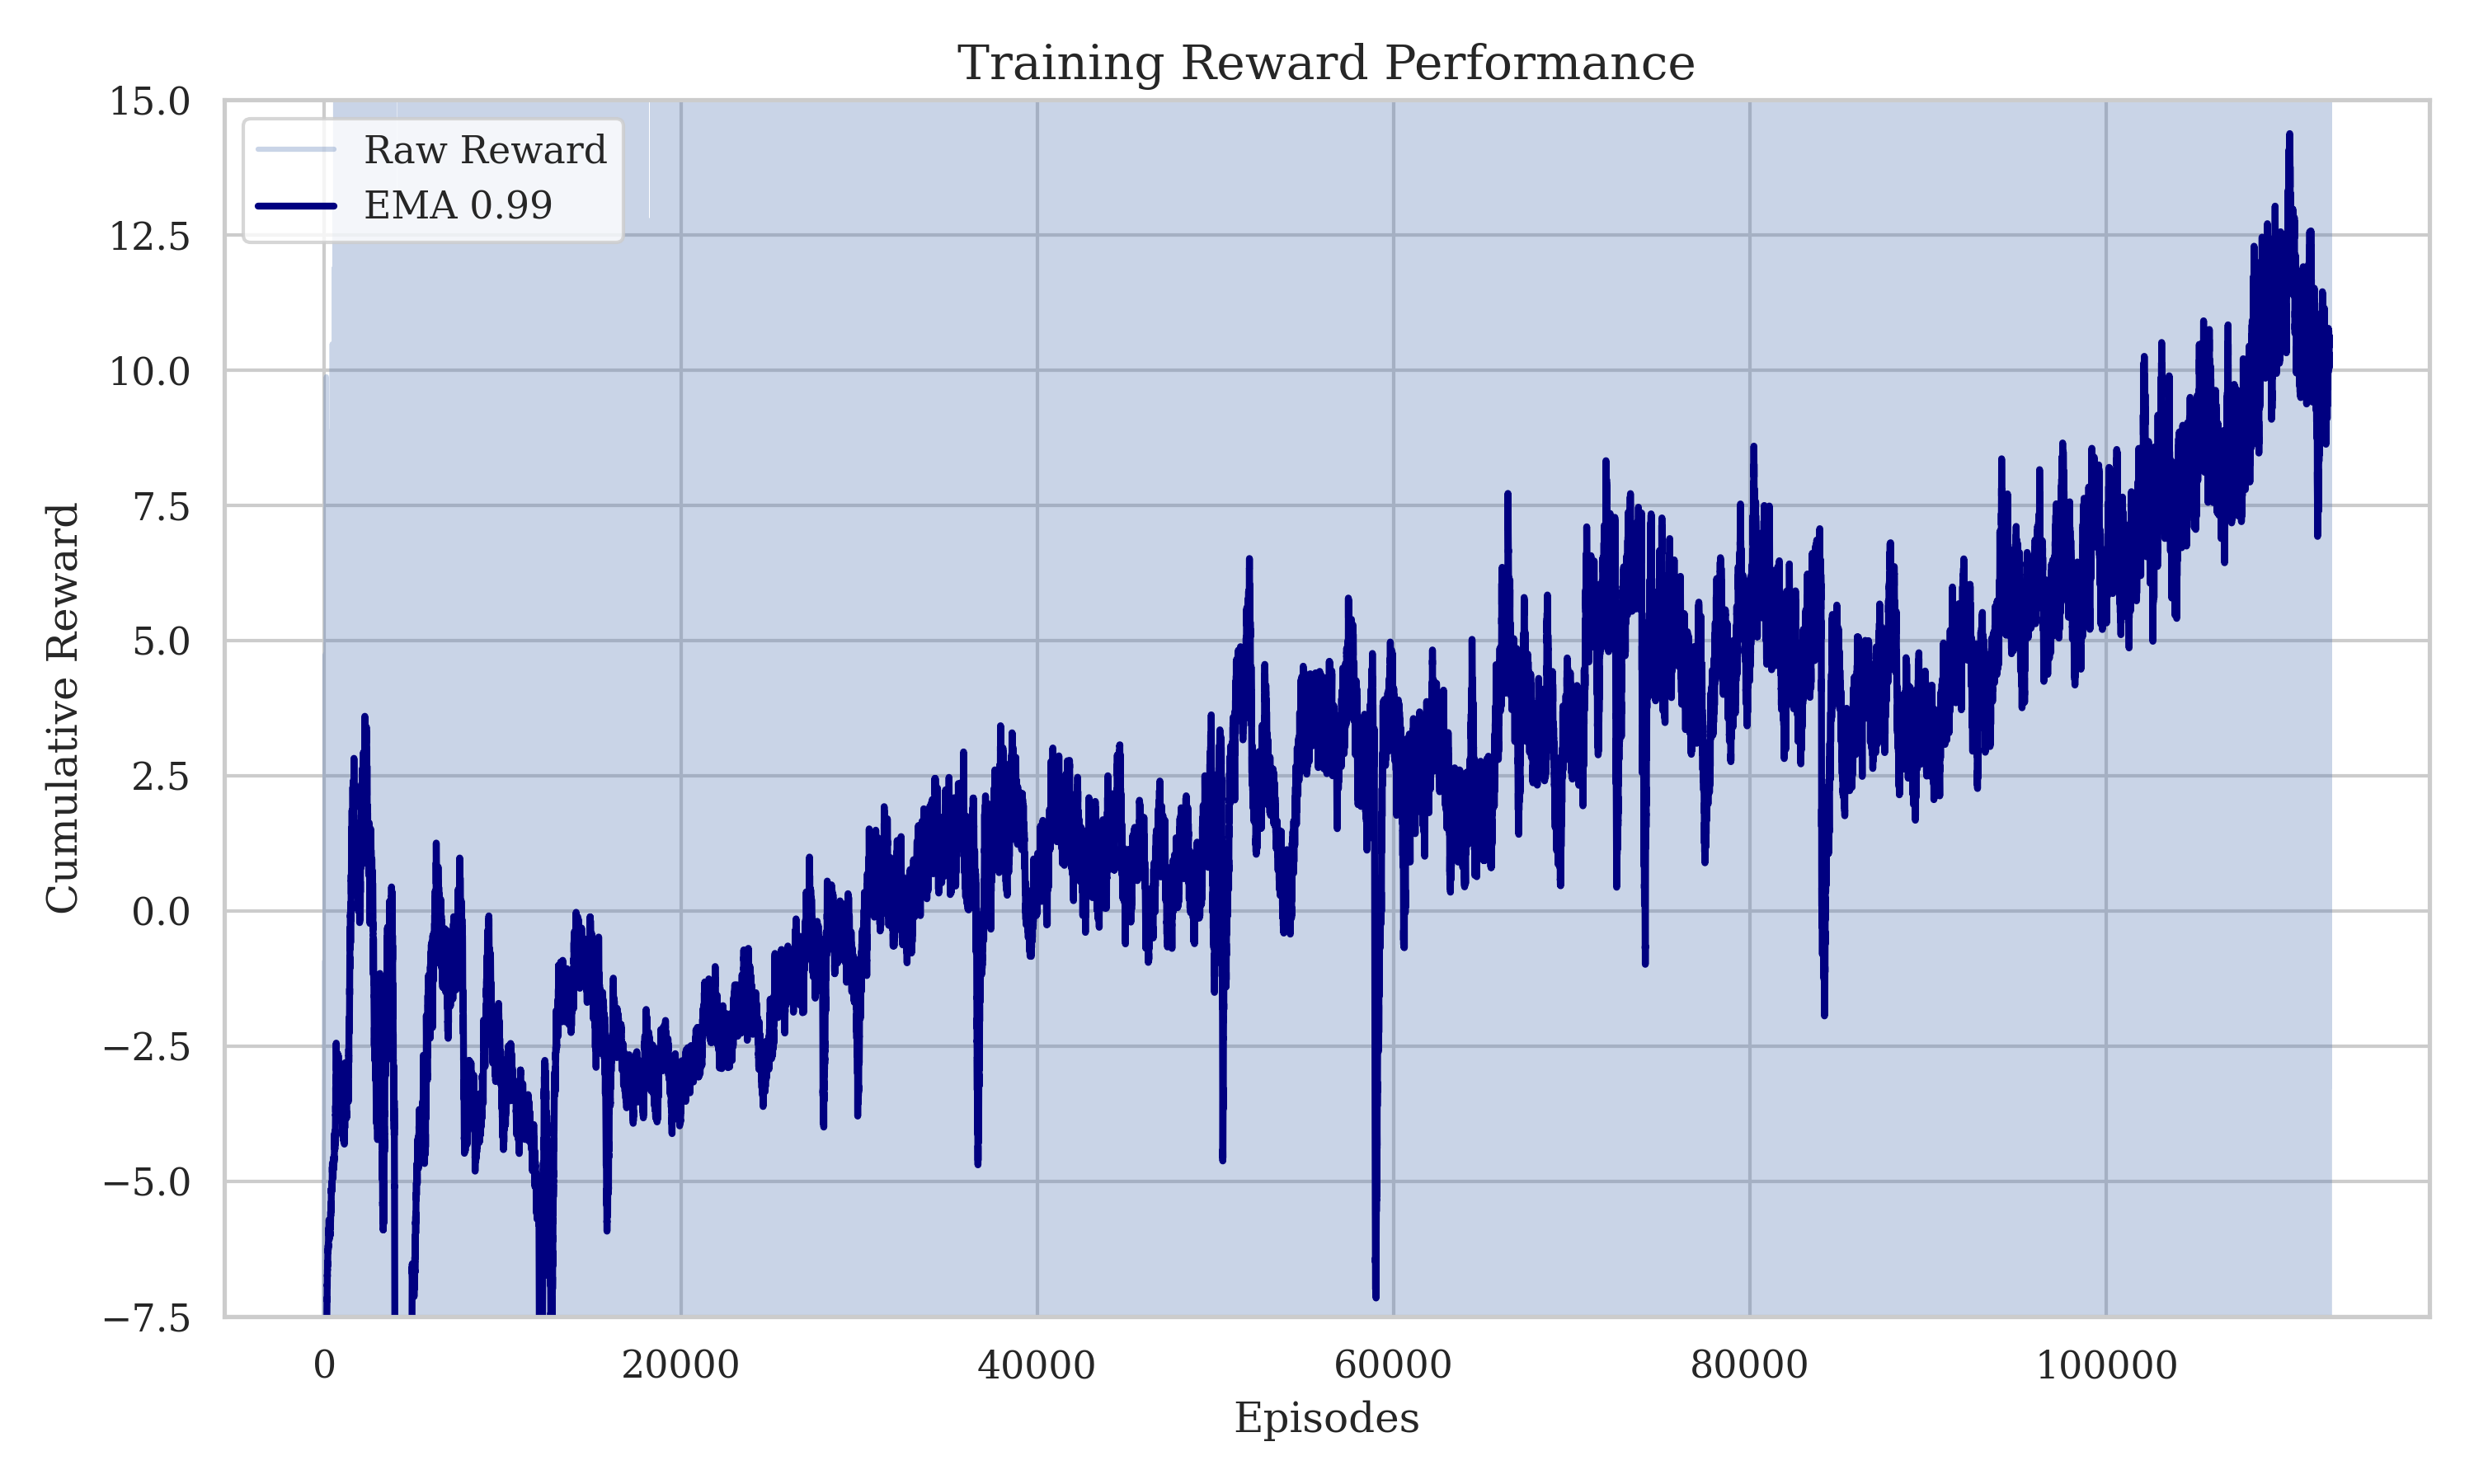
\includegraphics[width=0.3\textwidth]{figures/train reward.png}
        \caption{Train Reward Curve}
        \label{fig:Train Reward Curve}
    \end{figure}

    \begin{figure}[htbp]
        \centering
        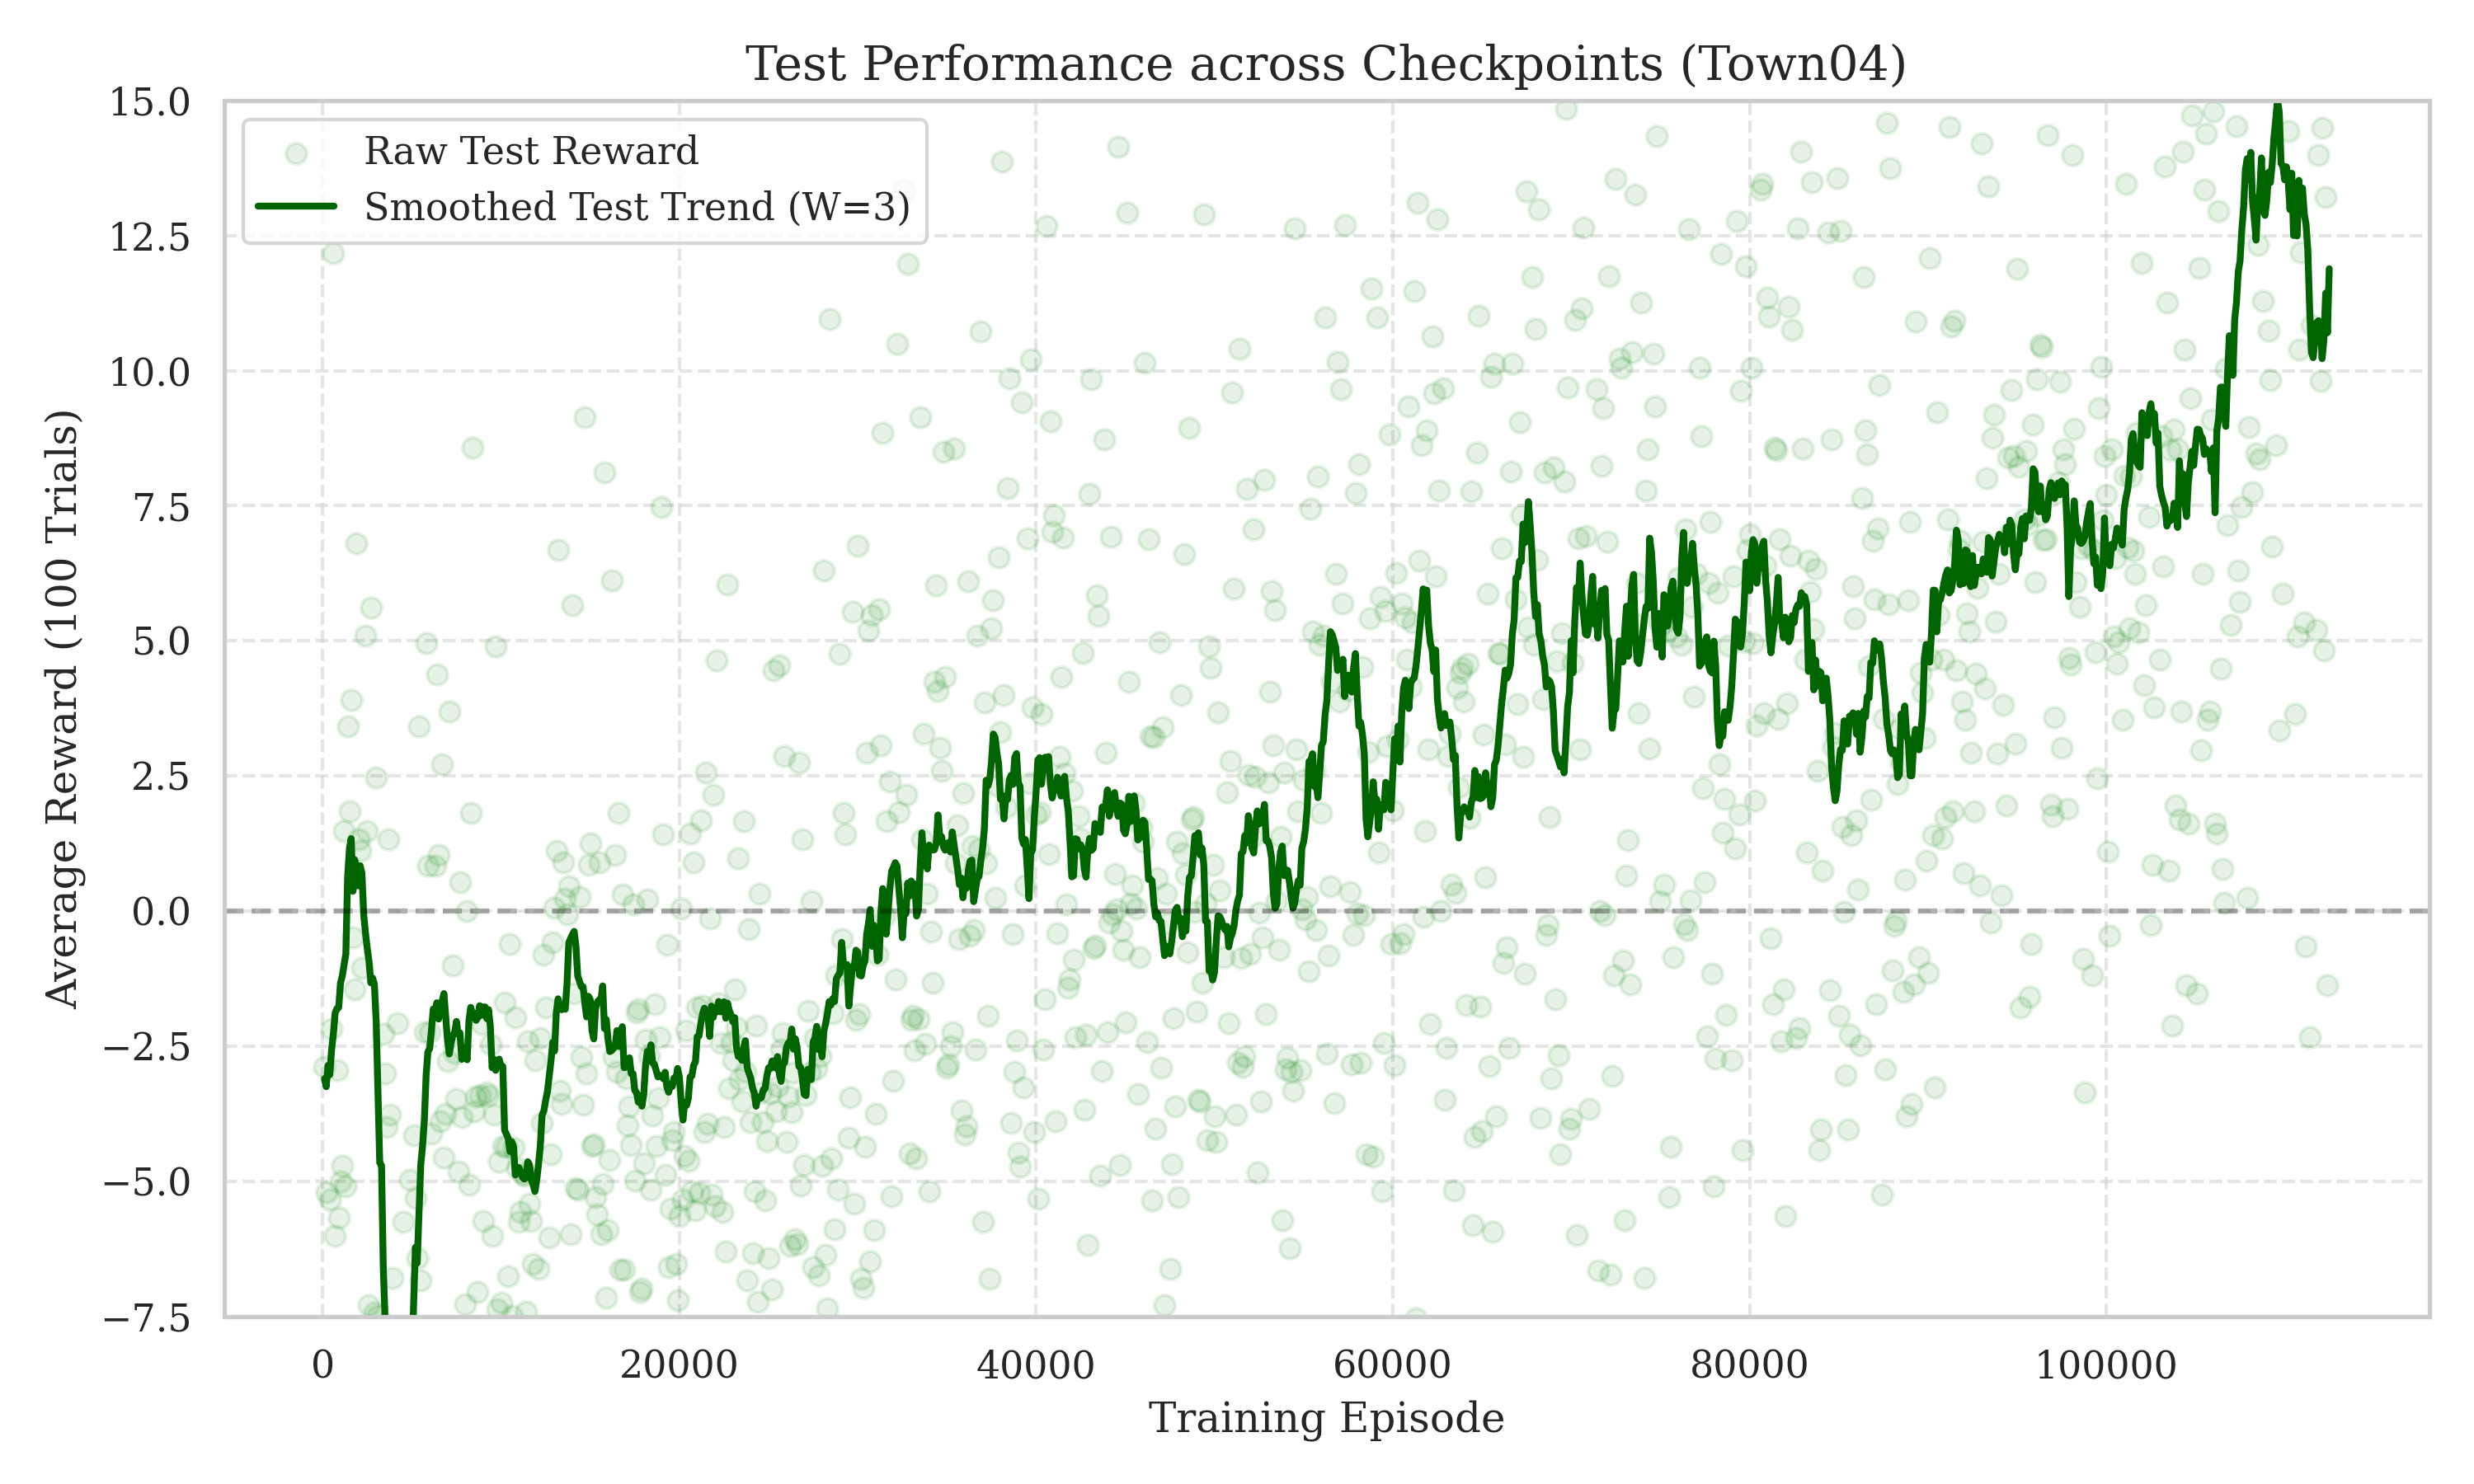
\includegraphics[width=0.3\textwidth]{figures/test reward.png}
        \caption{Test Reward Curve}
        \label{fig:Test Reward Curve}
    \end{figure}

    To evaluate the learning efficiency of ViT-SAC, we recorded the training and evaluation rewards at each checkpoint.

    As shown in \ref{fig:Train Reward Curve} and \ref{fig:Test Reward Curve} , the reward drops significantly in the initial stage of the model. This phenomenon mainly stems from the agent's initial interaction with the simulation environment after completing behavior cloning pre-training, frequently triggering penalties such as collisions and lane incursions when facing unfamiliar states. To avoid collisions or lane incursions, the model adopted a passive strategy to avoid significant penalties. However, due to the introduction of a stopping penalty mechanism, the cumulative penalty of inaction outweighed the risk of exploration. Combined with the inherent maximum entropy mechanism of the SAC algorithm, the agent began to actively explore. Subsequently, the training reward showed a continuous upward trend, rising from a negative baseline to the positive region. Although accompanied by spikes due to high-risk actions, the Double Critic network achieved rapid correction. In the later stages of training, the training reward reached a peak of 15, marking the end of the final training phase of this study.

    The reward curves of the testing and training phases in this study are similar. The environmental parameters are the same for the testing and training phases. The only difference is that the entropy mechanism used for random exploration is turned off in the evaluation phase, and a purely deterministic policy is used for action output.

    \begin{table}[htbp]
    \centering
    \caption{Best Checkpoint Performance Metrics}
    \label{tab:performance_metrics}
    \begin{tabular}{cccc}
    \toprule
    \textbf{Episode} & \textbf{Success Rate} & \textbf{Collision Rate} & \textbf{Offroad Rate} \\ \midrule
    108299 & 58 & 28 & 14\\
    110999 & 50 & 34 & 16\\
    109399 & 48 & 36 & 16\\
    108699 & 44 & 48 & 8\\
    107699 & 42 & 44 & 14\\
    \bottomrule
    \end{tabular}
    \end{table}

    These are the final results of this study. The testing method involved conducting five random intersection tests on each checkpoint. Then, the 25 best-performing checkpoints were selected for more detailed testing. In the detailed testing phase, 50 intersections were randomly selected to obtain a more realistic assessment of the checkpoints' capabilities. The above are the five best-performing checkpoints in this study. The best-performing checkpoint was 108299, with a success rate of 58\%, a collision rate of 28\%, and a road exit rate of 14\%.
% % !TeX root = ../main.tex

\section{Conclusion}
    This study successfully combines the ViT model and the SAC algorithm to address the ViT data hunger problem. The best-performing checkpoint in this study achieved a 58\% success rate and a 28\% collision rate at unsignalized intersections. Its performance approaches that of leading studies in this field (e.g., \cite{x_zhang_integrating_2025}, with a success rate of 67.3\%). While there are some gaps compared to other studies using non-front-view image input, the front-view image input used in this study has greater deployment potential. Although the success rate is still far from practical application, this study fully validates the feasibility of this technical approach.

    Due to computational resource constraints, the current model network size and training time are still relatively limited, containing only two Transformer encoding blocks and four frames of 56x168 pixel visual signal input. Future research can expand the network capacity and increase the number of pixels by stacking more Transformer layers. This alignment strategy conforms to the large model parameter scaling theorem validated in \cite{wu_rewarddance_2025}. We firmly believe that with a greater investment of computing resources, this framework can unleash even greater performance potential.
    

\clearpage
\printbibliography 

\section*{BIOGRAPHIES OF AUTHORS}
\small
\textbf{Jun Xuan Ng} is currently a student/researcher... He can be contacted at email: your.email@example.com. [cite: 214, 222]

\end{document}